\documentclass{article}[12pt]
\usepackage[a4paper, margin=1in]{geometry}

% packages
%   formatting
%\usepackage[utf8]{inputenc}
\usepackage{url}
\usepackage{hyperref}
\hypersetup{
    colorlinks=true,
    linkcolor=blue,
    filecolor=magenta,      
    urlcolor=blue}
\usepackage{xcolor}
%\usepackage[T1]{fontenc}
%\usepackage{lmodern}
\usepackage{float}
%   math
\usepackage{amsmath}
\usepackage{amssymb}
%\usepackage{bbm}

%\usepackage{mathptmx}
%\usepackage{verbatim}
%\usepackage{bm}
%   figures, tables, ...
\usepackage{algpseudocode}
\usepackage{algorithm}
\usepackage{graphicx}
\usepackage{booktabs}
\usepackage{makecell}
%\usepackage{multirow}%http://ctan.org/pkg/multirow

\usepackage{amsthm}
\newtheorem{theorem}{Theorem}[section]
\newtheorem{corollary}{Corollary}[theorem]
\newtheorem{lemma}[theorem]{Lemma}

% python
\usepackage{listings}
\definecolor{darkgreen}{rgb}{0,0.6,0}
\lstdefinestyle{Python}{
    showstringspaces=false,
    language        = Python,
    basicstyle      = \small\ttfamily,
    morekeywords = {as},
    keywordstyle    = \color{blue},
    stringstyle     = \color{darkgreen},
    commentstyle    = \color{darkgreen}\ttfamily,
	breaklines = true,
	postbreak=\text{$\hookrightarrow$\space},
	% style >>> and ... 
	%   see: https://tex.stackexchange.com/questions/326655/make-a-keyword-in-listings-enviorment
	alsoletter = {>,.} ,
    morekeywords = [2]{>>>,...},
    keywordstyle = [2]\color{cyan}\bfseries}

% bibliograpy
\usepackage{biblatex}
\addbibresource{ags.bib}
\addbibresource{main.bib}

% macros
\input ags.tex
\newcommand{\bvarepsabs}{\boldsymbol{\varepsilon}_\text{abs}}
\newcommand{\bvarepsrel}{\boldsymbol{\varepsilon}_\text{rel}}
\newcommand{\varepsabs}{\varepsilon_\text{abs}}
\newcommand{\varepsrel}{\varepsilon_\text{rel}}

\newcommand{\JRComment}[1]{{\color{violet}#1}}
\newcommand{\FJHComment}[1]{{\color{purple}Fred:  #1}}
\newcommand{\CDHJComment}[1]{{\color{royal blue}#1}}

\DeclareMathOperator{\Order}{{\mathcal O}}

% metadata
\title{Monte Carlo for Vector Functions of Integrals}
\author{Aleksei Sorokin, Jagadeeswaran Rathinavel}
\date{\today}


\begin{document}

\maketitle

\begin{abstract}
Monte Carlo methods present an efficient approach for approximating the expected value of a random variable. Algorithms exist to adaptively sample the random variable until a user defined error tolerance is satisfied with high probability. This work describes an extension of such methods, which supports adaptive sampling to satisfy error criteria for vector functions of multiple expectations. Although several functions involving multiple expectations are being evaluated, only one random sequence is required, albeit sometimes of larger dimension than the underlying randomness. These enhanced Monte Carlo and Quasi-Monte Carlo algorithms are implemented in the QMCPy Python package with support for vectorized, economical, and parallel function evaluation. We exemplify these capabilities on problems from machine learning and global sensitivity analysis.
\end{abstract}

\tableofcontents

\newpage

\section{Introduction}

\FJHComment{You may want to start importing this into the conference proceedings styles so that you can adapt to them sooner rather than later.

To cut down on the number of pages, you may want to refer readers to a demo of your code on the QMCPy website.  The editors may have trouble compiling the LaTeX of the book with your source code listings definitions.

%It is better not to have just one subsubsection of a subsection.
}

Theoretical developments, stopping criteria, and implementations of Monte Carlo (MC) methods often focus on approximating a scalar expectation $\mu = \bbE[f(\bX)]$, where $\bX \sim \calU[0,1)^d$ encapsulates the randomness of a simulation $f: [0,1)^d \to \bbR$. However, many quantities of interest $\bs \in \bbR^{\bd_{\bs}}$, which we call \emph{combined solutions}, may be formulated as functions of expectations $\bmu = \bbE[\bf(\bX)] \in \bbR^{\bd_{\bmu}}$, which we call \emph{individual solutions}. Now the simulation $\bf: [0,1)^{d} \to \bbR^{\bd_{\bmu}}$ produces a multi-dimensional array with vector shape $\bd_{\bmu}$ while $\bX \sim \calU[0,1)^d$ as in the scalar function setting. The multi-dimensional array of combined solutions is produced from the multi-dimensional array of individual solutions via a \emph{combining function} $\bC: \bbR^{\bd_{\bmu}} \to \bbR^{\bd_{\bs}}$ so that 
\begin{equation}
    \bs = \bC(\bmu).
    \label{eq:comb_from_indv}
\end{equation}
For example, approximating
\begin{itemize}
    \item an $(a \times b)$ matrix of expectations sets $\bC$ to the identity function and $\bd_{\bs} = \bd_{\bmu} = (a,b)$;
    \item the Bayesian posterior mean requires the ratio of expectations so that $s = C(\mu_1,\mu_2) = \mu_1/\mu_2$, $d_s = 1$, and $d_{\bmu} = 2$;
    \item $c$ closed and total sensitivity indices for global sensitivity analysis may require $\bd_{\bs} = (2,c)$ and $\bd_{\bmu} = (2,3,c)$ to formulate $s_{ij} = C_{ij}(\bmu) =  \mu_{i3j}/(\mu_{i2j}-\mu_{i1j}^2)$ for $i \in \{1,2\}$ and $j \in \{1,\dots,c\}$.
\end{itemize}
These examples are further detailed in Section \ref{sec:examples}.

This article generalizes \cite{adaptive_qmc} to develop Algorithm \ref{algo:MCStoppingCriterion}, an efficient and adaptive method for approximating combined solutions $\bs$ to within a user-specified error tolerance and uncertainty threshold. The algorithm utilizes existing MC  methods that, given an appropriate set of sampling nodes and their corresponding function evaluations, produce error bounds on individual solutions that hold with a desired confidence. Examples of scalar-bounding MC methods include \cite{cubmcg,cubqmclattice,cubqmcsobol,cubqmcbayes_thesis,cubqmcbayeslattice} with robust implementations in the GAIL MATLAB library \cite{ChoEtal21a,hickernell2018monte}. Interval arithmetic is used to propagate these individual solution bounds to bounds on the combined solutions which can be used both to test if the error criterion has been met and determine optimal combined solution approximations. 

\JRComment{Please mention any prior work in vectorized Monte Carlo}

The resulting vectorized MC algorithms for combined solutions are implemented into the open source QMCPy Python package \cite{QMCPy} which is distributed on both GitHub and PyPI. The implementations incorporate shared samples, multi-dimensional vectorization, parallel computation, and economical function evaluation to enable fast, efficient approximations. Section \ref{sec:examples} also provides use cases in QMCPy with all examples being fully reproducible in \AGSNote{cite \url{https://github.com/QMCSoftware/QMCSoftware/blob/mc_vec/demos/vectorized_qmc.ipynb}}.

The remainder of the article is organized as follows. Section \ref{sec:MCM} provides a brief overview of scalar MC including both Crude and Quasi-MC methods. More detailed accounts of this mature field are available in \cite{niederreiter1992random,mcbook}. Section \ref{sec:Existing_QMC_Methods} outlines various MC methods for determining error bounds on a scalar individual solution. Section \ref{sec:comb_sol_approx} determines how to set uncertainty levels for individual bounds based on a desired uncertainty for a scalar combined solution and how to propagated bounds from individual to combined solutions using interval arithmetic \cite{interval_analysis}. Section \ref{sec:opt_comb_sol_sc} derives a stopping criterion and optimal approximation for a scalar combined solution based on a user-specified uncertainty threshold and error metric map. Vectorization to a multi-dimensional array of combined solutions is described Section \ref{sec: Vectorized Implementation} with special care taken to enable economical function evaluation. This section also details Algorithm \ref{algo:MCStoppingCriterion} which provides a framework for extending existing MC methods to accommodate approximating multi-dimensional arrays of combined solutions. Section \ref{sec:examples} presents examples from machine learning and global sensitivity analysis utilizing our implementation in QMCPy. We conclude with a brief summary in Section \ref{sec:conclusions}.   

\section{Scalar Monte Carlo Methods} \label{sec:MCM}

As mentioned previously, MC methods are well-suited to approximate a scalar expectation $\mu = \bbE[f(\bX)]$ where $\bX \sim \calU[0,1)^d$ contains the randomness of a simulation $f: [0,1)^{d} \to \bbR$. While the standard uniform choice for $\bX$ may seem restrictive, a variety of random variables are compatible in this framework after an appropriate transformation. For example, if $\mu = \bbE[g(\bT)]$ for $\bT \sim \calN(\boldsymbol{m},\boldsymbol{\Sigma})$ and some $g: \bbR^{d} \to \bbR$, then $\mu = \bbE[f(\bX)]$ for  $f(\bx)=g(\boldsymbol{A}\Phi^{-1}(\bx)+\boldsymbol{m})$ where $\boldsymbol{\Sigma}=\boldsymbol{A}\boldsymbol{A}^T$ and $\Phi^{-1}$ \FJHComment{You may want $\boldsymbol{\Phi}^{-1}$ since it is a vector-valued function.} is the inverse CDF of a standard normal distribution acting element wise. More details on such variable transformations can be found in \cite{QMCSoftware} along with examples of how to utilize the default transforms available in QMCPy.

MC methods often approximate $\mu$ by the sample average of $f$ evaluated at some nodes $\bx_1,\dots,\bx_n \in [0,1)^d$. We denote this approximation by  
\begin{equation}
    \label{eq:mcapprox}
    \hat{\mu} = \frac{1}{n}\sum_{i=1}^n f(\bx_i) \approx \bbE[f(\bX)] = \mu. 
\end{equation}
\emph{Crude Monte Carlo} (CMC) methods choose the sampling nodes to be independent and identically distributed (IID), that is $\bx_1,\dots,\bx_n \simiid \calU[0,1)^{d}$. For CMC, the absolute approximation error $\lvert \mu - \hat{\mu} \rvert$ is $\calO(n^{-1/2})$. 

\emph{Quasi-Monte Carlo} (QMC) methods choose the sampling nodes in a dependent manner to avoid the gaps and clusters observed in IID nodes. Discrepancy measures quantify how close the empirical distribution of $\{\bx_i\}_{i=1}^n$ is to the standard uniform distribution. The Koksma-Hlawka inequality bounds the absolute approximation error by the star discrepancy of $\{\bx_i\}_{i=1}^n$ times the variation of $f$ in the sense of Hardy and Krause \cite{dick2013high}. Other discrepancy-variation pairings are also available, see \cite{hickernell1998generalized} for an overview. While it is often impractical to determine if $f$ has bounded variation, such inequalities indicate that using low discrepancy (LD) sequences in place of IID sequences can boost performance for nicely behaved $f$. A number of LD sequences exist that achieve a discrepancy of $\calO(n^{-1+\delta})$ for any $\delta > 0$. These LD sequences are the backbone QMC methods. When $f$ has bounded variation, this rate upper bounds the absolute error of QMC methods making them significantly faster than CMC methods. Oftentimes, even if $f$ has infinite variation, QMC methods will still outperform CMC methods despite a lack of theoretical justification. 


The QMC methods in this article utilize randomized LD sequences that are extensible in both dimension and number of samples without sacrificing the $\calO(n^{-1+\delta})$ discrepancy rate. Randomization ensures, with probability $1$, that $\bx_1,\dots,\bx_n \in (0,1)^d$ and that the LD sequence does not badly match the integrand. Extensiblity enables algorithms to adaptively increase the number of points used to estimate $\hat{\mu}$ without needing to discard previous function evaluations. Digital sequences and integration lattices are two popular choices for LD sequences. Constructions exist for both that support randomization and extensible designs. Figure \ref{fig:ld_seqs} contrasts IID points with LD sequences implemented in base $2$ as is often done for computational efficiently.

\begin{figure}[t]
    \centering
    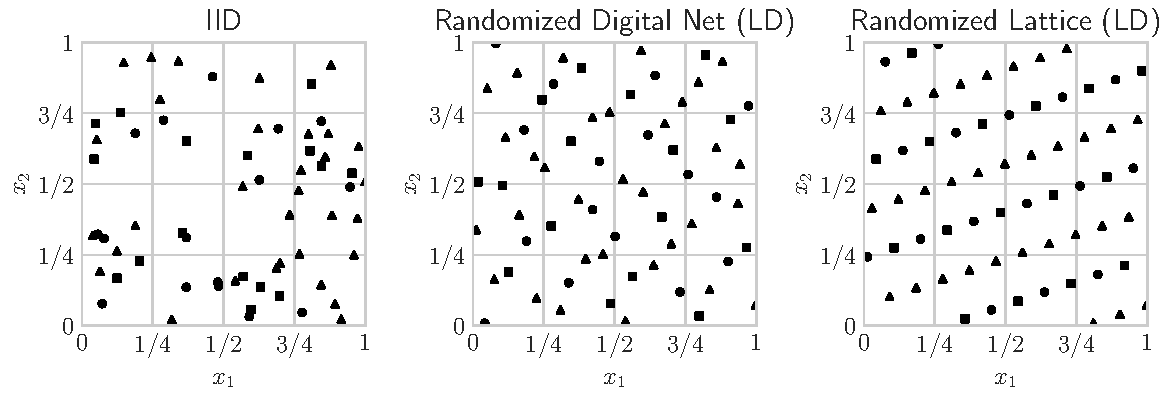
\includegraphics[width=\textwidth]{figs/ld_seqs.pdf}
    \caption{Contrast of IID points with randomized, extensible LD sequences. The first $2^4$ points of each sequence are squares, the next $2^4$ points are circles, and the $2^5$ points following that are triangles. Notice the gaps and clusters in the IID sequence contrasted with the more even coverage of LD sequences. Also notice that as the sample size is doubled the extensible LD sequences fills in the gaps left by previous nodes.}
    \label{fig:ld_seqs}
\end{figure}

% \begin{algorithm}[t]
%     \caption{$\texttt{Gen.Lattice}(R,n)$}
%     \label{algo:Gen.Lattice}
%     \begin{algorithmic}
%     \Require $R \in \bbN$, the number of independent randomizations.
%     \Require $n = 2^m \in \bbN$, the number of nodes in the lattice sequence.
%     \\ \hrulefill
%     \State fix $\bv \in \bbN^{d}$, a carefully chosen Lattice generating vector, see \cite{cools2006constructing,hickernell2000extensible} for details. 
%     \State draw $\boldsymbol{\Delta}_1,\dots,\boldsymbol{\Delta}_R \simiid \calU(0,1)^{d}$
%     \For{$i \gets 0,\dots,n-1$}
%         \State $t \gets \sum_{k=1}^m 2^{-k}i_k$ where $i = \sum_{k=1}^m 2^{k-1} i_k$ 
%         \State $\bx_{i+1} \gets (t\bv) \mod \boldsymbol{1}$
%         \For{$r \gets 1,\dots, R$}
%             \State $\bx_{i+1}^{(r)} \gets (\bx_{i+1}+\boldsymbol{\Delta}_r) \mod \boldsymbol{1}$
%         \EndFor
%     \EndFor
%     \State \Return $\{\{\bx_i^{(r)}\}_{i=1}^n\}_{r=1}^R$
%     \end{algorithmic}
% \end{algorithm}

\section{Scalar Monte Carlo Approximation Error}\label{sec:Existing_QMC_Methods}

This section discusses some existing CMC and QMC methods for approximating error bounds on the scalar individual solution $\mu$. Specifically, given $n$ samples $\bx_1,\dots,\bx_n$ and corresponding function evaluations $f(\bx_1),\dots,f(\bx_n)$, we discuss methods for determining lower bound $\mu^-$ and upper bound $\mu^+$ so that $\mu \in [\mu^-,\mu^+]$ with probability greater than or equal to some desired threshold $1-\alpha^{(\mu)}$. Table \ref{table:qmcpy_sc} compares the error bounding methods discussed in the remainder of this section.

\begin{table}[t]
\centering
\begin{tabular}{r c c c c c c}
    QMCPy Class Name & MC Type & Point Sets & Error Bounds \\
    \hline
    \texttt{CubMCCLT} \cite{cubmcg} & CMC & \texttt{IID} & Probabilistic \\
    \texttt{CubQMCRep} \cite{mcbook} & QMC & \texttt{LD} & Probabilistic \\
    \texttt{CubQMCNetG} \cite{cubqmcsobol} & QMC & \texttt{DigitalNetB2} & Deterministic \\
    \texttt{CubQMCLatticeG} \cite{cubqmclattice} & QMC & \texttt{Lattice} & Deterministic \\
    \texttt{CubQMCBayesNetG} \cite{cubqmcbayes_thesis} & QMC &  \texttt{DigitalNetB2} & Bayesian \\
    \texttt{CubQMCBayesLatticeG} \cite{cubqmcbayeslattice} & QMC & \texttt{Lattice} & Bayesian \\
    \hline
\end{tabular}
\caption{A comparison of select stopping criterion classes available in QMCPy. \emph{MC Type} indicates wheather an algorithm is Crude Monte Carlo (CMC) or Quasi-Monte Carlo (QMC). \emph{Point Sets} indicate classes of compatible sequences in QMCPy. For example, \texttt{CubQMCRep} is compatible with any low discrepancy (\texttt{LD}) sequence including base 2 digital nets (\texttt{DigitalNetB2}) and integration lattices (\texttt{Lattice}). However, \texttt{CubQMCNetG} is only compatible with \texttt{DigitalNetB2} sequences and will not work with \texttt{Lattice} or other LD sequences. \emph{Error Bounds} specify the method of error estimation as discussed throughout this section. Deterministic error bounds hold with probability $1$ i.e. for any $\alpha^{(\mu)} \in (0,1)$. Probabilistic and Bayesian error bounds are tailored to the choice of $\alpha^{(\mu)}$.}
\label{table:qmcpy_sc}
\end{table}

\begin{description}
    \item[\texttt{CubMCCLT}] When $\bx_1,\dots,\bx_n$ are IID and $f$ has finite variance, the Central Limit Theorem may provide a heuristic $1-\alpha^{(\mu)}$ confidence interval for $\mu$ by setting $\mu^\pm = \hat{\mu} \pm Z_{\alpha^{(\mu)}/2}\sigma/\sqrt{n}$. Here $Z_{\alpha^{(\mu)}/2}$ is the inverse CDF of a standard normal distribution at $1-\alpha^{(\mu)}/2$, and $\hat{\mu}$ is the sample average of function evaluations as in \eqref{eq:mcapprox}. The standard deviation of $f(\bX)$ is the generally unknown quantity $\sigma$ which may be approximated by the unbiased estimator $\hat{\sigma} = \sqrt{1/(n-1)\sum_{i=1}^n(f(\bx_i)-\hat{\mu})^2}$, perhaps multiplied by an inflation factor $C>1$ for a more conservative estimate. Thus the heuristic error bounds on $\mu$ are
    \begin{equation*}
        \mu^\pm = \hat{\mu} \pm \frac{CZ_{\alpha^{(\mu)}/2}\hat{\sigma}}{\sqrt{n}}
        \label{eq:clt_mu_bounds}.
    \end{equation*}
    These bounds only hold as $n \to \infty$ so they cannot guaranteed to satisfy the desired uncertainty. 
    
    \citeauthor{cubmcg} modify this idea in \cite{cubmcg} to accommodate  finite $n$ and provide error bounds that are guaranteed to satisfy the uncertainty threshold. Their two-step method relies on the Berry-Esseen inequality and the assumption that $f$ lies in a cone of functions with known, bounded kurtosis. This robust method is not immediately compatible with the framework of this article but has been implemented into the QMCPy stopping criterion class \texttt{CubMCG} to approximate a scalar individual solution.
    \item[\texttt{CubQMCRep}] This method utilizes IID randomizations of a LD sequence and then derives bounds based on the IID sample averages. Specifically, suppose $\{\bx_i^{(1)}\}_{i=1}^n,\dots,\{\bx_i^{(R)}\}_{i=1}^n$ are $R$ IID randomizations of an LD point set. Then one may compute the $R$ IID sample averages $\hat{\mu}_r = \frac{1}{n} \sum_{i=1}^n f(\bx_i^{(r)})$ for $r = 1,\dots,R$. Similar to what was done for \texttt{CubMCCLT}, one may then compute 
    $$\hat{\mu} = \frac{1}{R} \sum_{r=1}^R \hat{\mu}_r \quad\text{and}\quad \hat{\sigma}_R = \sqrt{\frac{1}{R-1}\sum_{i=1}^R(\hat{\mu}_r - \hat{\mu})^2}$$
    to produce heuristic bounds  
    $$\mu^\pm = \hat{\mu} \pm \frac{C T_{\alpha^{(\mu)}/2,R-1} \hat{\sigma}_R}{\sqrt{R}}.$$
    Here $C>1$ is still an inflation factor and we now use $T_{\alpha^{(\mu)}/2,R-1}$, the inverse CDF of Student's-$t$ distribution with $R-1$ degrees of freedom, instead of $Z_{\alpha^{(\mu)}/2}$.
    A more careful treatment of this heuristic method is available in either \cite[Chapter 17]{mcbook} or \cite{qmc4pde_preprint}. 
    \item[\texttt{CubQMC\{Net,Lattice\}G}] \citeauthor{cubqmclattice} developed algorithms in \cite{adaptive_qmc} that track the decay of Fourier coefficients based on a single randomized LD sequence i.e. $R=1$. These algorithms provide deterministic error bounds on $\mu$ for functions in a cone parameterized by the decay rate of the Walsh coefficients for digital sequences \cite{cubqmcsobol} or the complex exponential Fourier coefficients for integration lattices \cite{cubqmclattice}. %In particular for \texttt{CubQMCLatticeG}, the cone comprises of functions whose Fourier series are absolutely convergent and whose true Fourier coefficients decay steadily as the wave-number tends to infinity.
    \item[\texttt{CubQMCBayes\{Net,Lattice\}G}] Another pair of QMC algorithms take a Bayesian approach to error estimation, again using only a single randomized LD sequence. Rather than assume the function lies within a cone, these algorithms assume the integrand is an instance of a Gaussian process. 
    %Alternatively, rather than assume the integrand is deterministic, these methods assume the integrand is an instance of a random Gaussian process.  
    Utilizing special kernels matched to LD sequences allows fast approximation of Gaussian process hyperparameters and provides tractable error estimation. These Bayesian QMC algorithms are also available for both digital nets \cite{cubqmcbayes_thesis} and integration lattices  \cite{cubqmcbayeslattice}. 
    %Similar to \texttt{CubQMC\{Net,Lattice\}G}, Fourier and Walsh transform coefficients are used respectively with Lattice and digital nets. But the coefficients are used to estimate credible intervals. Thus it provides much stronger theoretical background. These algorithms need to estimate shape and scale parameters to parameterize the covariance kernels, which are to be searched using optimization techniques, leading to greater computational cost. 
\end{description}

\JRComment{Is there any default recommendation if the user does not have any knowledge about the integrand?}

We first recommend using the  \texttt{CubQMC\{Net,Lattice\}G} QMC algorithms if the function's Fourier coefficients are expected to be well behaved and the function has low evaluation cost. For functions with larger evaluation cost and low dimension, we recommend using  \texttt{CubQMCBayes\{Net,Lattice\}G}. While these algorithms require additional overhead for optimizing Gaussian Process hyperparameters, they tend to be more sample efficient than \texttt{CubQMC\{Net,Lattice\}G}. \texttt{CubQMCRep} accommodates a larger class of functions compared to the other QMC algorithms with the drawback of providing heuristic bounds and often requiring more samples to achieve the same error. If QMC is not suitable for the problem, \texttt{CubMCCLT} may be used, again with the caution of producing heuristic bounds which lack theoretical justification.

Digital nets may generally be preferred to lattice point sets as the later often requires the function be periodic. While periodizing transforms are available to any function, such transforms may destroy smoothness properties previously enjoyed by the function. See \cite[Chapter 16]{mcbook} for more details on periodizing transforms for lattice rules.

%The Bayesian cubature algorithms are not recommended where the integrand's Fourier coefficients are not expected to be well behaved. Also not recommended for very dimensional integrands for which the parameters search will be computationally prohibitive. One advantage of using the digital-net cubature is the integrand does not have to be periodic in the unit cube $[0, 1)^d$ whereas the lattice based cubature algorithm expects the integrand to be periodic. 

% \paragraph{Computational cost of \texttt{CubQMCBayes\{Net,Lattice\}G }:}
% The Bayesian cubature requires a computational cost of
% \begin{equation} \label{eqn:OuralgoCost}
%     \mathcal{O}\bigl(n \$(f) + N_{\opt}[n\$(C) + n \log(n)] \bigr),
% \end{equation} 
% where $\$(f)$ is the cost of one integrand value, $\$(C)$ is the cost of a single covariance kernel value,  $\Order(n \log(n))$ is the cost of a fast Fourier transform, and $N_{\opt}$ is an upper bound on the number of optimization steps required to choose the hyperparameters. If function evaluation is expensive, e.g., the output of a computationally intensive simulation, or if $\$(f) = \Order(d)$ for large $d$, then $\$(f)$ might be similar in magnitude to $N_{\opt} \log(n)$ in practice.  Typically, $\$(C) = \Order(d)$.  Note that the $\Order(n \log(n))$ contribution is $d$ independent.

\section{Individual Uncertainties and Bound Propagation for a Scalar Combined Solution} \label{sec:comb_sol_approx}

\FJHComment{It would help to have a connecting sentence or two at the start and/or end of each section to tell the reader where you are going next.  E.g., In this section, we connect errors in individual solutions to errors in combined solutions.}

The MC and QMC algorithms in the previous section may be vectorized in a straightforward manner to attain error bounds $[\bmu^-,\bmu^+]$ on a multi-dimensional array of individual solutions $\bmu \in \bbR^{\bd_{\bmu}}$ so that 
\begin{equation}
    P(\mu_{\bk} \in [\mu_{\bk}^-,\mu_{\bk}^+]) \geq 1-\alpha_{\bk}^{(\bmu)}  \qquad \text{for any multi-index }\boldsymbol{1} \leq \bk \leq \bd_{\bmu}.
    \label{eq:indv_prob_bounds}
\end{equation}
%for any multi-index $\boldsymbol{1} \leq \bk \leq \bd_{\bmu}$. 
Here $\balpha^{(\bmu)} \in (0,1)^{\bd_{\bmu}}$ is a multi-dimensional array of individual uncertainty levels which are set to 
\begin{equation}
    \alpha_{\bk}^{(\bmu)} = \frac{\alpha^{(s)}}{\prod(\bd_{\bmu})}
    \label{eq:alpha_mu_from_alpha_s} \qquad \text{for all }\boldsymbol{1} \leq \bk \leq \bd_{\bmu}.
\end{equation}
%for all $\boldsymbol{1} \leq \bk \leq \bd_{\bmu}$. 
In the above, $\prod(\bd_{\bmu})$ is the number of elements in a $\bbR^{\bd_{\bmu}}$ array [ \JRComment{which array is referred here?}] and $\alpha^{(s)} \in (0,1)$ is the desired uncertainty for the bounds $[s^-,s^+]$ on the scalar combined solution $s$. In this setting, Boole's inequality \cite{boole1847mathematical} implies that whenever \eqref{eq:indv_prob_bounds} holds we have
\begin{equation}
    P(\bmu \in [\bmu^-,\bmu^+]) \geq 1-\alpha^{(s)}.
    \label{eq:indv_prob_bounds_all}
\end{equation} 

Recall from \eqref{eq:comb_from_indv} that $s = C(\bmu)$ where, in this case, $C: \bbR^{\bd_{\bmu}} \to \bbR$. To propagate individual bounds $[\bmu^-,\bmu^+]$ to combined bounds $[s^-,s^+]$, one defines interval arithmetic \cite{interval_analysis} functions $C^-,C^+: \bbR^{\bd_{\bmu}} \times \bbR^{\bd_{\bmu}} \to \bbR$ so that
\begin{equation}
    \begin{aligned}
    s^- &= C^-(\bmu^-,\bmu^+) &&= \min_{\bmu \in [\bmu^-,\bmu^+]} C(\bmu) \\
    s^+ &= C^+(\bmu^-,\bmu^+) &&= \max_{\bmu \in [\bmu^-,\bmu^+]} C(\bmu).
    \end{aligned}
    \label{eq:C_minus_C_plus}
\end{equation}
Table \ref{table:elementary_ops_Cpm} provides examples of such interval arithmetic functions for some basic operations. \JRComment{The next line is not clear:} Finally, under settings \FJHComment{assumptions?} \eqref{eq:alpha_mu_from_alpha_s} and \eqref{eq:C_minus_C_plus} we have that  \eqref{eq:indv_prob_bounds} implies \eqref{eq:indv_prob_bounds_all} implies
$$\qquad  P(s \in [s^-,s^+]) \geq 1-\alpha^{(s)}$$
as desired.

\begin{table}[t]
\begin{tabular}{r  c  c}
    $s=C(\bmu)$ & $s^- = C^-(\bmu^-,\bmu^+)$ & $s^+ = C^+(\bmu^-,\bmu^+)$ \\
    \hline
    $\mu_1+\mu_2$ & $\mu_1^-+\mu_2^-$ & $\mu_1^++\mu_2^+$ \\
    $\mu_1-\mu_2$ & $\mu_1^--\mu_2^+$ & $\mu_1^+-\mu_2^-$ \\
    $\mu_1 \cdot \mu_2$ & $\min(\mu_1^-\mu_2^-,\mu_1^-\mu_2^+,\mu_1^+\mu_2^-,\mu_1^+\mu_2^+)$ & $\max(\mu_1^-\mu_2^-,\mu_1^-\mu_2^+,\mu_1^+\mu_2^-,\mu_1^+\mu_2^+)$ \\
    $\mu_1 / \mu_2$ & $\begin{cases} -\infty, & 0 \in [\mu_2^-,\mu_2^+] \\ \min\left(\frac{\mu_1^-}{\mu_2^-},\frac{\mu_1^+}{\mu_2^-},\frac{\mu_1^-}{\mu_2^+},\frac{\mu_1^+}{\mu_2^+}\right), & 0 \notin [\mu_2^-,\mu_2^+] \end{cases}$ & $\begin{cases} \infty, & 0 \in [\mu_2^-,\mu_2^+] \\ \max\left(\frac{\mu_1^-}{\mu_2^-},\frac{\mu_1^+}{\mu_2^-},\frac{\mu_1^-}{\mu_2^+},\frac{\mu_1^+}{\mu_2^+}\right), & 0 \notin [\mu_2^-,\mu_2^+] \end{cases}$ \\
    $\min(\mu_1,\mu_2)$ & $\min(\mu_1^-,\mu_2^-)$ & $\min(\mu_1^+,\mu_2^+)$ \\
    $\max(\mu_1,\mu_2)$ & $\max(\mu_1^-,\mu_2^-)$ & $\max(\mu_1^+,\mu_2^+)$ \\
    \hline
\end{tabular}
\caption{Bound propagation functions for elementary operations on individual solutions.}
\label{table:elementary_ops_Cpm}
\end{table}

\section{Stopping Criterion and Approximation for a Scalar Combined Solution} \label{sec:opt_comb_sol_sc}

Let $h^{(\varepsilon)}: \bbR \to \bbR^+$ be an error metric dependent on some error threshold $\varepsilon$ so that the stopping criterion is met if and only if the combined solution approximation $\hat{s}$ satisfies 
\begin{equation}
    \lvert s-\hat{s} \rvert \leq h^{(\varepsilon)}(s), \qquad \forall\; s \in [s^-,s^+].
    \label{eq:sc_raw}
\end{equation}
Theorem \ref{thm:shat_opt} below determines an optimal $\hat{s}$ and an equivalent condition to \eqref{eq:sc_raw} when $h^{(\varepsilon)}$ is metric map i.e Lipschitz continuous with constant less than or equal to $1$. Compatible error metric options include
\begin{subequations}
\begin{align}
    h^{(\varepsilon)}(s) & = \varepsilon \quad &&\text{absolute error satisfied}, \label{eq:h_abs}\\
    h^{(\varepsilon)}(s) & = \lvert s \rvert \varepsrel \quad &&\text{relative error satisfied}, \label{eq:h_rel}\\
    h^{(\varepsilon)}(s) &= \max\left(\varepsabs,\lvert s \rvert \varepsrel \right) \quad &&\text{absolute or relative error satisfied, and } \label{eq:h_abs_or_rel} \\
    h^{(\varepsilon)}(s) &= \min\left(\varepsabs,\lvert s \rvert \varepsrel \right) \quad &&\text{absolute and relative error satisfied.} \label{eq:h_abs_and_rel}
\end{align}
\end{subequations}
\begin{theorem} \label{thm:shat_opt}
    Suppose that  $h^{(\varepsilon)}$ satisfies the metric map condition
    $$\lvert h^{(\varepsilon)}(s_1) - h^{(\varepsilon)}(s_2) \rvert \leq \lvert s_1 - s_2 \rvert \qquad \text{for all } s_1,s_2 \in \bbR.$$
    Then error criterion  \eqref{eq:sc_raw} holds if and only if 
    \begin{equation}
        s^+-s^- \leq h^{(\varepsilon)}(s^-)+h^{(\varepsilon)}(s^+).
        \label{eq:sc}
    \end{equation}
    Furthermore, the choice of 
    \begin{equation}
        \hat{s} = \frac{1}{2}\left[s^-+s^++h^{(\varepsilon)}(s^-)-h^{(\varepsilon)}(s^+)\right].
        \label{eq:shat_opt}
    \end{equation}
    minimizes $\max_{s \in [s^-,s^+]} \lvert s - \hat{s} \rvert -h^{(\varepsilon)}(s)$ for any choice of $s^{\pm}$ with $s^- < s^+$.
\end{theorem}

\begin{proof}
    Define $g(s,\hat{s})=\lvert s - \hat{s} \rvert -h^{(\varepsilon)}(s)$. We first establish that the maximum of $g(\cdot,\hat{s})$ over $[s^-,s^+]$ occurs at the boundaries for any real $\hat{s}$.  
    
    If  $s^- \leq s \leq \hat{s}$ it follows that 
    $$g(s^-,\hat{s})-g(s,\hat{s}) = \lvert s^- - \hat{s} \rvert -h^{(\varepsilon)}(s^-) - \lvert s - \hat{s} \rvert  + h^{(\varepsilon)}(s) \geq s - s^- - \lvert h^{(\varepsilon)}(s)-h^{(\varepsilon)}(s^-) \rvert \geq 0,$$
    and if $\hat{s} \leq s \leq s^+$ then 
    $$g(s^+,\hat{s})-g(s,\hat{s}) = \lvert s^+ - \hat{s} \rvert -h^{(\varepsilon)}(s^+) - \lvert s - \hat{s} \rvert  + h^{(\varepsilon)}(s) \geq s^+ - s - \lvert h^{(\varepsilon)}(s)-h^{(\varepsilon)}(s^+) \rvert \geq 0.$$
    This means that $g(\cdot,\hat{s})$ attains its maximum at either $s^-$ or $s^+$ so that
    \begin{equation*}
        \max_{s \in [s^-,s^+]} g(s,\hat{s}) = \max_{s \in \{s^-,s^+\}} g(s,\hat{s}).
    \end{equation*}
    
    Next, we find the optimal choice of $\hat{s}$.  The function $g(s^-,\cdot)$ is monotonically decreasing to the left of  $s^-$ and monotonically increasing to the right of $s^-$. Similarly, $g(s^+,\cdot)$ is monotonically decreasing to the left of $s^+$ and monotonically increasing to the right of $s^+$. This means that the optimal choice of $\hat{s}$ to minimize $\max_{s \in \{s^-,s^+\}} g(s,\hat{s})$ lies in $[s^-,s^+]$ and satisfies $g(s^-,\hat{s}) = g(s^+,\hat{s})$, that is, 
    $$\hat{s} - s^- - h^{(\varepsilon)}(s^-) = s^+ - \hat{s} - h^{(\varepsilon)}(s^+).$$
    Solving for the optimal value of $\hat{s}$ leads to \eqref{eq:shat_opt}.
    
    For this optimal $\hat{s}$, 
    $$2 \max_{s \in [s^-,s^+]} g(s,\hat{s}) =  s^+  -  s^-  - h^{(\varepsilon)}(s^-) - h^{(\varepsilon)}(s^+).$$
    The error criterion is equivalent to $\max_{s \in [s^-,s^+]} g(s,\hat{s}) \le 0 $.  This can only hold under condition  \eqref{eq:sc}. 
\end{proof}

\section{MC Algorithm for Multi-Dimensional Combined Solutions} \label{sec: Vectorized Implementation}

In the previous section we assumed that a multi-dimensional array of individual solutions $\bmu \in \bbR^{\bd_{\bmu}}$ were used to compute a scalar combined solution $s \in \bbR$. We now relax these assumptions to enable approximation of multi-dimensional combined solutions $\bs \in \bbR^{\bd_{\bs}}$. The optimal approximation $\hat{\bs} \in \bbR^{\bd_{\bs}}$ and stopping criterion may still be computed by element-wise versions of by \eqref{eq:shat_opt} and \eqref{eq:sc}. 

To enable economical function evaluation, the user may define a dependency function
$$\bD: \tfset^{\bd_{\bs}} \to \tfset^{\bd_{\bmu}}$$ 
which maps error criterion flags on the combined solutions to flags on individual solutions. These individual flags indicate which outputs the integrand is required to compute in the next iteration. Take a simple example where  $\bs=\bmu$ so $\bC$ and $\bD$ are the identity function. At some iteration suppose the combined flag at multi-index $\boldsymbol{1} \leq \bl \leq \bd_{\bs}$ is $\True$, indicating the combined, and therefore individual, solution at index $\bl$ has been sufficiently approximated. Then in the next iteration, the function does not need to compute outputs at index $\bl$.

Moreover, $\bD$ may be used to compute individual uncertainty levels $\balpha^{(\bmu)}$ by determining which and how many individual solution contribute to a combined solution. Specifically, we may adapt \eqref{eq:alpha_mu_from_alpha_s} so that 
$\alpha_{\bk}^{(\bmu)}$ is the reciprocal of the maximum number of dependent individual solutions across all combined solutions which include $\bk$ as a dependency.

Algorithm \ref{algo:MCStoppingCriterion} details the adaptive, vectorized MC procedure developed throughout this article. Notice that the implementation does not require specifying $\bC$ despite its use in deriving the necessary $\bC^-,\bC^+$ inputs. The cost of this algorithm is concentrated in evaluating the function at an IID or LD sequence. In practice, the run time may be reduced if the users simulation code can take advantage of not having to compute all outputs at every iteration or through parallel evaluation if the simulation is costly to evaluate.

\begin{algorithm}[t]
    \caption{Adaptive, Vectorized Monte Carlo Algorithm}
    \label{algo:MCStoppingCriterion}
    \begin{algorithmic}
    \Require $\bf: (0,1)^d \to \bbR^{\bd_{\bmu}}$, the simulation where $\bmu = \bbE[\bf(\bX)]$ for $\bX \sim \calU[0,1)^d$.
    \Require $\balpha^{(\bs)} \in (0,1)^{\bd_{\bs}}$, the desired uncertainty levels for combined solutions so the bounds result in
    \begin{equation}
        P(s_{\bl} \in [s_{\bl}^-,s_{\bl}^+]) \geq 1-\alpha^{(\bs)}_{\bl} \quad \text{for any}\quad \; \boldsymbol{1} \leq \bl \leq \bd_{\bs}.
        \label{eq:comb_bounds_per_bl}
    \end{equation}
    If the user wants bounds $[\bs^-,\bs^+]$ so that $P(\bs \in [\bs^-,\bs^+]) \geq 1-\alpha$ for some $\alpha \in (0,1)$ then set $\alpha_{\bl}^{(\bs)} = 1/\prod(\bd_{\bs})$ in the spirit of \eqref{eq:alpha_mu_from_alpha_s}.
    \Require $\bC^-,\bC^+: \bbR^{\bd_{\bmu}} \times \bbR^{\bd_{\bmu}} \to \bbR^{\bd_{\bs}}$, vectorized interval arithmetic functions as in \eqref{eq:C_minus_C_plus} so that \eqref{eq:indv_prob_bounds_all} implies \eqref{eq:comb_bounds_per_bl}.
    \Require $h^{(\varepsilon_{\bl})}_{\bl}: \bbR \to \bbR^+$ for $\boldsymbol{1} \leq \bl \leq \bd_{\bl}$, for example \eqref{eq:h_abs}, \eqref{eq:h_rel}, \eqref{eq:h_abs_or_rel}, or \eqref{eq:h_abs_and_rel}.
    \Require $\bD: \tfset^{\bd_{\bs}} \to \tfset^{\bd_{\bmu}}$, a dependency function mapping stopping criterion flags for the combined solutions to flags for individual solutions. 
    \Require A generator of IID or LD sequences.
    \Require A scalar CMC or QMC algorithm compatible with the sequence generator(s) which produces individual bounds to within a desired uncertainty threshold based on samples from the sequence(s) and their corresponding function evaluations. See the methods in Section \ref{sec:Existing_QMC_Methods}.
    \Require $m_0 \in \bbN$, where $2^{m_0}$ is the initial number of samples.
    \\ \hrulefill
    \State $n_\text{start} \gets 0$ \Comment{lower index in node sequence(s)}
    \State $n_\text{end} \gets 2^{m_0}$ \Comment{upper index in node sequence(s), \emph{not} inclusive}
    \State $\bb^{(\bmu)} \gets \False^{\bd_{\bmu}}$ \Comment{flags on individual solutions}
    \State $\bb^{(\bs)} \gets \False^{\bd_{\bs}}$ \Comment{flags on combined solutions}
    \State Set $\balpha^{(\bmu)}$ based on $\balpha^{(\bs)}$ as described in Section \ref{sec: Vectorized Implementation}
    \While{$b_{\bl}^{(\bs)} = \False$ for some $\boldsymbol{1} \leq \bl \leq \bd_{\bs}$} \Comment{Some combined solution has not been sufficiently bounded}
        \State Generate nodes from the IID or LD sequence(s) from index $n_\text{start}$ to $n_\text{end}$
        \State Evaluate $\bf$ at the new nodes from the previous step to produce outputs where $\bb^{(\bmu)}=\textbf{\False}$ \\ \Comment{may be done in parallel if advantageous}
        \State Update $\bmu^-$ and $\bmu^+$ based on the new nodes and function evaluations using the scalar CMC or QMC algorithms applied element-wise 
        \State $[\bs^-,\bs^+] = \left[\bC^-(\bmu^-,\bmu^+),\bC^+(\bmu^-,\bmu^+)\right]$ 
        \State $\hat{s}_{\bl} \gets \frac{1}{2}\left[s_{\bl}^-+s_{\bl}^++h^{(\bvarepsilon)}_{\bl}(s_{\bl}^-)-h^{(\bvarepsilon)}_{\bl}(s_{\bl}^+)\right]$ for $\boldsymbol{1} \leq \bl \leq \bd_{\bs}$ \Comment{\eqref{eq:shat_opt} applied element-wise}
        \State $\bb^{(\bs)} \gets \textbf{Boolean}\left(\bs^+-\bs^- < \bh_{\bvarepsilon}(\bs^-)+\bh_{\bvarepsilon}(\bs^+)\right)$ \Comment{\eqref{eq:sc} applied element-wise}
        \State $\bb^{(\bmu)} \gets \bD\left(\bb^{(\bs)}\right)$
        \State $n_\text{start} \gets n_\text{end}$
        \State $n_\text{end} \gets 2n_\text{start}$
    \EndWhile
    \State \Return $\hat{\bs},[\hat{\bs}^-,\hat{\bs}^+]$
    \end{algorithmic}
\end{algorithm}

\section{Examples} \label{sec:examples}

The following examples are implemented into the object oriented QMCPy framework. Throughout the remainder of this section we assume the QMCPy package \cite{QMCPy} has been imported alongside the numerical package NumPy \cite{numpy} via the following Python commands. 
\lstinputlisting[caption={Imports},style=Python,label={py:imports}]{python/imports.txt}
The four main abstract classes in QMCPy are the 
\begin{itemize}
    \item \emph{discrete distribution} class for generating IID or LD sequences;
    \item \emph{true measure} class for facilitating variable transforms to adapt randomness to the standard uniform;
    \item \emph{integrand} class specifying the function of the true measure we want to take the expectation of; 
    \item \emph{stopping criterion} class with an \texttt{integrate} method to adaptively sample the integrand until the stopping criterion is satisfied as in Algorithm \ref{algo:MCStoppingCriterion}.
\end{itemize}
Each MC problem must instantiate a subclass of each of the four abstract classes in a nested fashion. 

As a simple example, let us compute the expected displacement and stress on a cantilever beam as defined in \cite{ simulationlib_cantilever}: 
\begin{align*}
    D(T_1,T_2,T_3) &= \frac{4l^3}{T_1 w t} \sqrt{\frac{T_2^2}{t^4} + \frac{T_3^2}{w^4}} \\ 
    S(T_1,T_2,T_3) &= 600\left(\frac{T_2}{wt^2} + \frac{T_3}{w^2t}\right).
    \label{eq:cantilever_beam}
\end{align*}
Here $l=100$, $w=4$, $t=2$ are constants and $T_1$, $T_2$, $T_3$ are independent Gaussian random variables with mean and standard deviation as defined as in the Table \ref{tab:cantilever_beam} below.
\begin{table}[t]
    \centering
    \begin{tabular}{r c c l}
        Gaussian Variable & mean & standard deviation & Description \\ 
        \hline \\
        $T_1$ & $2.9 \times 10^7$ & $1.45 \times 10^6$ & Young's modulus of beam material \\
        $T_2$ & $500$ & $100$ & horizontal load on beam \\
        $T_3$ & $1000$ & $100$ & vertical load on beam
    \end{tabular}
    \caption{Variable descriptions for the cantilever beam function.}
    \label{tab:cantilever_beam}
\end{table}
Listing \ref{py:simpleex} uses QMCPy to approximates $s_1 = \mu_1 = \bbE[D(\bT)]$ and $s_2 = \mu_2 = \bbE[S(\bT)]$ where the identity functions for $\bC^-$, $\bC^+$, and $\bD$ are defaulted to. Notice that \texttt{CustomFun} is constructed with $g$, a function of the true measure $\bT$, rather than $f$, a function of MC compatible $\bX$ \FJHComment{I do not understand what his means.}. The variable transform taking $g$ to $f$ is performed automatically by QMCPy without explicit specification from the user. Here the absolute or relative error metric \eqref{eq:h_abs_or_rel} is defaulted to.
\lstinputlisting[caption={Simple QMCPy Example},style=Python,label={py:simpleex}]{python/simple_ex.txt}
For more details on the QMCPy framework see \cite{QMCSoftware}.

\subsection{Vectorized Acquisition Functions for Bayesian Optimization}

Bayesian optimization (BO) is a sequential optimization technique that attempts to find the global maximum of a black box function $\tilde{f}: (0,1)^{d} \to \bbR$. It is assumed that $\tilde{f}$ is expensive to evaluate, so we must strategically select sampling locations that maximize some utility or acquisition function. At a high level, BO 
\begin{enumerate}
    \item iteratively samples $\tilde{f}$ at locations maximizing the acquisition function,
    \item updates a Gaussian process surrogate based on these new observations,
    \item updates the acquisition function based on the updated surrogate,
    \item and repeats until the budget for sampling $\tilde{f}$ has been expired.
\end{enumerate}
More details on Bayesian optimization including formulas for the posterior mean and covariance may be found in \cite{frazier2018tutorial}.

Concretely, suppose we have already sampled $\tilde{f}$ at $\bz_1,\dots,\bz_{N} \in [0,1]^{d}$ to collect data $\calD=\{(\bz_i,y_i)\}_{i=1}^N$ where $y_i = \tilde{f}(\bz_i)$. BO may then fit a Gaussian process surrogate $\tilde{g}$ to data $\calD$. The next $q$ sampling locations may then be chosen to maximize  an acquisition function $\alpha$ based on the surrogate $\tilde{g}$ so that 
\begin{equation}
    \begin{pmatrix}\bz_{N+1} \\ \vdots \\ \bz_{N+q}\end{pmatrix} = \argmax_{\bZ \in [0,1]^{(q,d)}}\alpha(\bZ).
    \label{eq:nextq}
\end{equation}
Many acquisition functions may be expressed as an expectation of the form
$$\alpha(\bZ) = \bbE\left[a(\by) \mid \by \sim \calN\left(\boldsymbol{m},\bSigma\right)\right]$$
where $\boldsymbol{m} \in \bbR^{q}$, $\bSigma \in \bbR^{(q, q)}$ are the posterior mean and covariance respectively of the Gaussian process at points $\bZ$. Here we focus on the q-Expected Improvement (qEI) acquisition function which uses 
$$a(\by) = \max_{1 \leq i \leq q} (y_i - y^*)_+$$
where $y^*= \max\left(y_1,\dots,y_N\right)$ is the current maximum and $(\cdot)_+ = \max(\cdot,0)$. 

Now, suppose that in \eqref{eq:nextq} we take the maximum argument from among a finite set of $q$-sized batches $\bZ_1,\dots,\bZ_c \in [0,1]^{(q, d)}$ so that 
\begin{equation}
    \begin{pmatrix}\bz_{N+1} \\ \vdots \\ \bz_{N+q}\end{pmatrix} = \argmax_{\bZ \in \{\bZ_1,\dots,\bZ_c\}}\alpha(\bZ).
    \label{eq:nextq_discrete}
\end{equation}
We may vectorize the acquisition function computations to 
\begin{equation}
    \bs = \bmu = \begin{pmatrix} \alpha(\bZ_1) \\ \vdots \\ \alpha(\bZ_c)\end{pmatrix} = \bbE\begin{pmatrix}a\left(\bA_1\Phi^{-1}(\bX)+\boldsymbol{m}_1\right) \\ \vdots \\ a\left(\bA_c\Phi^{-1}(\bX)+\bm_c\right)\end{pmatrix}
    \label{eq:bs_qei}
\end{equation}
where $\bX \sim \calU(0,1)^q$ and $\Phi^{-1}$ is the inverse CDF of the standard Gaussian taken element wise. Now $\bm_i$, $\bSigma_i = \bA_i\bA_i^T$ are the posterior mean, covariance respectively of the Gaussian process at $\bZ_i$ so that 
$$\bA_i\Phi^{-1}(\bX)+\boldsymbol{m}_i \sim \calN\left(\bm_i,\bSigma_i\right)$$
for $i=1,\dots,c$.

Since the quantity of interest is simply the vector of expectations in \eqref{eq:bs_qei}, one may set $\bC$, $\bC^-$, $\bC^+$, and $\bD$ to appropriate identity functions. The process described above is visualized in Figure \ref{fig:bo_qei} for $d=1$ and $q=2$. Notice the optimal point trades off exploiting parts of the domain where performant samples have already been observed and  exploring parts of the domain where the Gaussian Process has large uncertainty.  As $q$ and/or $d$ grow, the number of candidates $c$ required for \eqref{eq:nextq_discrete} to be a good discrete approximation of \eqref{eq:nextq} grows rapidly and therefore rendering such non-greedy acquisition functions intractable for even moderate values of $q$ or $d$.

\begin{figure}[t]
    \centering
    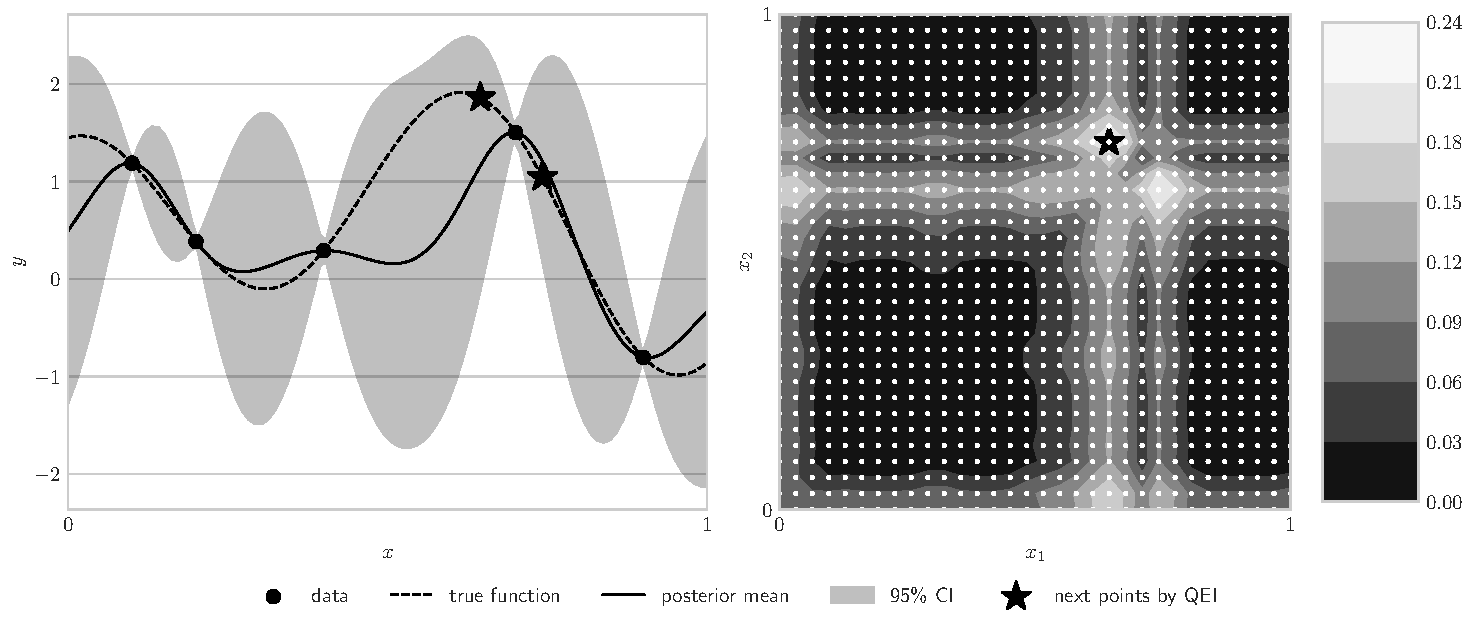
\includegraphics[width=\textwidth]{figs/gp.pdf}
    \caption{First, the true function has been sampled at the data points shown in the left panel. Next, a Gaussian Process is fit to the data points to approximate the true function, also shown in the left panel. With $q=2$, a fine grid of candidates is chosen in $[0,1]^{2}$ and depicted in the right panel. The vectorized MC algorithm is then used to approximate the acquisition function value at each of the candidate grid points. These approximations are made into a contour plot in the right panel. The discrete argument maximum among these approximations on the fine grid is the next size $q$ batch of points by qEI. These next points for sequential optimization are visualized in both the right and left panels. }
    \label{fig:bo_qei}
\end{figure}

\subsection{Bayesian Posterior Mean}

The Bayesian framework combines prior knowledge of unknown parameters $\bTheta$ with observational data and a likelihood function $\rho$ to construct an informed, model-aware posterior distribution on $\bTheta$. Suppose we have a dataset of observations $\by = (y_1,\dots,y_{N})$ taken at IID locations $\bz_1,\dots,\bz_{N}$ respectively. Then Bayes' rule may be used to write the posterior density of $\bTheta$ as 
$$P\left(\btheta \mid \by \right) = \frac{P(\by \mid \btheta) P(\btheta)}{P\left(\by\right)} = \frac{\prod_{i=1}^{N} \rho(y_i \mid \btheta) P(\btheta)}{\bbE\left[\prod_{i=1}^{N} \rho(y_i \mid \btheta)\right]}.$$
Here the expectation is taken with respect to the prior distribution on $\bTheta$ with density $P(\btheta)$, and $P\left(\by \mid \bS \right)$ is the likelihood density which factors into the product of likelihoods $\rho(y_i \mid \bS)$ since the observations are IID. 

A useful quantity of interest is the posterior mean of $\bTheta$. In this example, the posterior mean is our combined solution $\bs$ which may be written as the ratio of expectations via
$$\bs = \bbE\left[\bTheta \mid \by\right] = \frac{\bbE\left[\bTheta \prod_{i=1}^{N} \rho(y_i \mid \bS)\right]}{\bbE\left[\prod_{i=1}^{N} \rho(y_i \mid \bTheta)\right]}.$$
As before, the expectations are taken with respect to the prior distribution on $\bTheta$. In the framework of this article $\bmu \in \bbR^{(2, d_{\bs})}$ where for $k=1,\dots,d_{\bs}$ we have 
$$\mu_{0k} = \bbE\left[\Theta_i \prod_{i=1}^{N} \rho(y_i \mid \bTheta)\right], \qquad \mu_{1k} = \bbE\left[\prod_{i=1}^{N} \rho(y_i \mid \bTheta)\right], \qquad \text{and} \qquad s_k = \frac{\mu_{0k}}{\mu_{1k}}.$$
While $\mu_{1k}$ is the same for all $1 \leq k \leq d_{\bs}$, we opt to keep separate denominator estimates for each coefficient. Defining $\bC^-$ and $\bC^+$ follow from vectorizing the quotient forms in Table \ref{table:elementary_ops_Cpm} while the dependency function $\bD: \tfset^{d_{\bs}} \to \tfset^{(2, d_{\bs})}$ may be defined by stacking row vectors of combined flags such that
$$\bD\left(\bb^{(\bs)}\right) = \begin{pmatrix} \bb^{(\bs)} \\ \bb^{(\bs)} \end{pmatrix}.$$
Maintaining only a single estimate of $\bbE\left[\prod_{i=1}^{N} \rho(y_i \mid \bTheta)\right]$ would require a different dependency function which removes economic function evaluation in favor of reduced storage. 

Consider Bayesian logistic regression as a concrete example. Here the dataset contains observations $y_i \in \{0,1\}$ at locations $\bz_i = \left(z_{i1},\dots,z_{i(d_{\bs}-1)},1\right)$ for $i=1,\dots,N$ where the last value is $1$ to accommodate an intercept term. The sigmoid likelihood function
$$\rho(y_i = 1 \mid \btheta) = \frac{\exp(\btheta.\bz_i)}{1+\exp(\btheta.\bz_i)}$$
may be used to yield
$$P(\by \mid \btheta) = \prod_{i=1}^N \left(\frac{\exp(\btheta.\bz_i)}{1+\exp(\btheta.\bz_i)}\right)^{y_i} \left(1-\frac{\exp(\btheta.\bz_i)}{1+\exp(\btheta.\bz_i)}\right)^{1-y_i} = \prod_{i=1}^N \frac{\exp(\btheta.\bz_i)^{y_i}}{1+\exp(\btheta.\bz_i)}.$$

Listing \ref{py:blr} performs Bayesian logistic regression in QMCPy
%on the Haberman's Survival Dataset retrieved from the UCI Machine Learning Repository \cite{uci_ml_repo}
. Here we use a normal prior $\bTheta \sim \calN(\bm,\bSigma)$ so that
$$P(\btheta) = \frac{\exp\left(-(\btheta-\bm)^T\bSigma^{-1}(\btheta-\bm)/2\right)}{\sqrt{(2\pi)^d\lvert \det(\bSigma)\rvert }}.$$
This example uses the absolute and relative error metric \eqref{eq:h_abs_and_rel}. Notice that the number of samples required to approximate each coefficient is different. 

\lstinputlisting[caption={Bayesian Logistic Regression},style=Python,label={py:blr}]{python/blr.txt}

% \subsubsection{Haberman's Dataset Example}

% Here we perform logistic regression on the Haberman's Survival Dataset retrieved from the UCI Machine Learning Repository \cite{uci_ml_repo}. This dataset concerns a study between 1958 and 1970 at the University of Chicago's Billings Hospital that tracked the survival of patients five years after undergoing treatment for breast cancer. Predictors include the age of patient at the time of operation, operation year after 1900 e.g. 65 is 1965, and number of positive auxiliary nodes detected. The binary response variable indicates the patients survival status five years after the operation. 

% We use 2/3 of the dataset for training and the remaining 1/3 for testing. The training set has 151 positive records and 54 negative records while the testing set has 74 positive records and 27 negative records. The class imbalance reflects the fact that most patients in the study survived longer than 5 years after the operation. Since we value identifying at risk patients, we seek models with a low number of false negative predictions i.e. we desire models with high recall. Table \ref{tab:lr_models} compares a Bayesian logistic model against logistic regression models fit with an Elastic net regularization penalty
% $$\min_{\bs,c} \left[\frac{1-\lambda}{2} \lVert \bs \rVert_2^2 + \lambda \lVert \bs \rVert_1+C\sum_{i=1}^N\log(\exp(-y_i(\bx_i.\bs+c))+1)\right]$$
% where $C>0$ constant and $\lambda \in [0,1]$ controls the trade-off between $l_1$ and $l_2$ regularization. The Elastic-Net models were fit using the scikit-learn Python package with the ``saga'' optimizer \cite{scikit-learn}. The Bayesian logistic regression model was fit with $\bvarepsabs=.05$, $\bvarepsrel=.5$, error metric $h$ matching \eqref{eq:h_abs_and_rel}. Note that the Bayesian logistic regression model has the highest test recall metric.  

% \begin{table}[t]
%     \centering
%     \begin{tabular}{l|rrrr|rrr}
%         Method &\multicolumn{4}{|c|}{Coefficients} &\multicolumn{3}{c}{Test Metrics \%}\\
%         {} &       Age &  1900 Year &  Auxiliary Nodes &  Intercept &  Accuracy &  Precision &   Recall \\
%         \midrule
%         % begin insert
%         Elastic-Net $\lambda=0.0$ & -1.23e-02 &   3.44e-02 &       -1.15e-01 &   1.99e-03 &     74.3 &      76.7 &   93.2 \\
%         Elastic-Net $\lambda=0.5$ & -1.20e-02 &   3.42e-02 &       -1.15e-01 &   2.03e-03 &     74.3 &      76.7 &   93.2 \\
%         Elastic-Net $\lambda=1.0$ & -1.18e-02 &   3.39e-02 &       -1.14e-01 &   2.06e-03 &     74.3 &      76.7 &   93.2 \\
%         Bayesian                & -4.14e-03 &   1.30e-01 &       -1.57e-01 &   8.03e-03 &     74.3 &      74.0 &  100.0 \\
%         % end insert
%         \bottomrule
%     \end{tabular}
%     \caption{Comparison of Logistic regression models for the Haberman dataset.}
%     \label{tab:lr_models}
% \end{table}

\subsection{Sensitivity Indices}

Sensitivity analysis quantifies how uncertainty in a functions output may be attributed to subsets of function inputs. Functional ANOVA (analysis of variance) decomposes an objective function $\tilde{f} \in L^2(0,1)^{d}$ into the sum of orthogonal functions $(\tilde{f}_u)_{u \subseteq 1:d}$. Here $1:d=\{1,\dots,d\}$ denotes the set of all dimensions and $\tilde{f}_u \in L^2(0,1)^{\lvert u \rvert}$ denotes a sub-function dependent only on inputs $\bx_u = (x_j)_{j \in u}$ where $\lvert u \rvert$ is the cardinality of $u$. By construction, these sub-functions sum to the objective function so that
\begin{equation}
    \tilde{f}(\bx) = \sum_{u \subseteq 1:d} \tilde{f}_u(\bx_u) 
    \label{eq:fanova}
\end{equation}
\cite[Appendix A]{mcbook}. The orthogonality of sub-functions enables the variance of $\tilde{f}$ to be decomposed into the sum of variances of sub-functions. Specifically, denoting the variance of $\tilde{f}$ by $\sigma^2$, we may write
\begin{equation*}
    \sigma^2 = \sum_{u \subseteq 1:d} \sigma^2_u
\end{equation*}
where $\sigma^2_u$ is the variance of sub-function $\tilde{f}_u$. The sub-variance $\sigma_u$ directly quantifies the variance of $\tilde{f}$ attributable to inputs $u \subseteq 1:d$.  The \emph{closed and total Sobol' indices},
\begin{equation*}
    \underline{\tau}_u^2 = \sum_{v \subseteq u} \sigma^2_v \quad \text{and} \quad 
    \overline{\tau}_u^2 = \sum_{v \cap u \neq \emptyset} \sigma^2_v,
    \label{eq:sobol_indices}
\end{equation*}
quantify the variance attributable to subsets of $u$ and subsets containing $u$ respectively. The \emph{sensitivity indices},
\begin{equation*}
    \underline{s}_u = \underline{\tau}_u^2/\sigma^2 \quad \text{and} \quad 
    \overline{s}_u = \overline{\tau}_u^2/\sigma^2,
    \label{eq:sensitivity_indices_og}
\end{equation*}
normalize the Sobol' indices to quantify the proportion of variance explained by a given subset of inputs. 

Suppose one is interested in computing the closed and total sensitivity indices of $\tilde{f}$ at $u_1,\dots,u_c \subseteq 1:d$.  Then we may choose the individual solutions $\bmu \in \bbR^{(2, 3, c)}$ and combined solutions $\bs \in \bbR^{(2, c)}$ so that for $j=1,\dots,c$
\begin{equation}
\begin{aligned}
    \mu_{11j} &= \underline{\tau}_{u_j}^2 = \int_{[0,1]^{2d}} f(\bx)[f(\bx_{u_j},\bz_{-{u_j}})-f(\bz)]\D\bx\D\bz \\
    \mu_{21j} &= \overline{\tau}_{u_j}^2 = \frac{1}{2}\int_{[0,1]^{2d}} [f(\bz)-f(\bx_u,\bz_{-{u_j}})]^2\D\bx\D\bz \\
    \mu_{12j} &= \mu_{22j} = \int_{[0,1]^{d}} f(\bx)\D\bx, \\
    \mu_{13j} &= \mu_{23j} = \int_{[0,1]^{d}} f^2(\bx)\D\bx, \\
    s_{1j} &= \underline{s}_{u_j} = \frac{\underline{\tau}_{u_j}^2}{\sigma^2} = \frac{\mu_{11j}}{\mu_{13j}-\mu_{12j}^2}, \\
    s_{2j} &= \overline{s}_{u_j} = \frac{\overline{\tau}_{u_j}^2}{\sigma^2} = \frac{\mu_{21j}}{\mu_{23j}-\mu_{22j}^2}.  
\end{aligned}
\label{eq:mu_si}
\end{equation}
Here the notation
\begin{equation*}
    (\bx_{u},\bz_{-u}) = \left(\begin{aligned}x_{j}, \quad & j \in u \\ z_{j}, \quad & j \notin u \end{aligned}\right)_{j=1}^{d}
\end{equation*}
denotes a point with inputs $u$ from $\bx$ and inputs $-u=(1:d)\cap u^c$ from $\bz$. In \eqref{eq:mu_si}, $\bmu_1$ and $\bmu_2$ contain values for the closed and  total sensitivity indices respectively; $\bmu_{11}$ and $\bmu_{21}$ contain the closed and total Sobol' indices respectively; $\bmu_{i2}$ and $\bmu_{i3}$ contain first and second moments respectively for $i \in \{1,2\}$, again opting for duplicated estimates to enable more economic function evaluation. For the combined solutions, $\bs_1$ contains closed sensitivity indices while $\bs_2$ contains contains total sensitivity indices. 

Bounds from individual to combined solutions may be propagated via $\bC^-,\bC^+:\bbR^{(2, 3, c)} \to \bbR^{(2, c)}$ defined for $i \in \{1,2\}$ and $j \in \{1,\dots,c\}$  by  
\begin{align*}
    C_{ij}^-(\bmu^-,\bmu^+) 
    &= \text{clip}\left(\min_{\bmu \in [\bmu^-,\bmu^+]} \frac{\mu_{i1j}}{\mu_{i3j}-\mu_{i2j}^2}\right) \\
    &= \begin{cases} 
        \text{clip}\left(\min\left(\frac{\mu_{i1j}^-}{\mu_{i3j}^+-\left(\mu_{i2j}^-\right)^2},\frac{\mu_{i1j}^-}{\mu_{i3j}^+-\left(\mu_{i2j}^+\right)^2}\right)\right), & \mu_{i3j}^- - \left(\mu_{i2j}^\pm\right)^2 >0 \\
        0, &\text{else}
    \end{cases} \\
    C_{ij}^+(\bmu^-,\bmu^+) 
    &= \text{clip}\left(\max_{\bmu \in [\bmu^-,\bmu^+]} \frac{\mu_{i1j}}{\mu_{i3j}-\mu_{i2j}^2}\right) \\
    &= \begin{cases} 
        \text{clip}\left(\max\left(\frac{\mu_{i1j}^+}{\mu_{i3j}^--\left(\mu_{i2j}^-\right)^2},\frac{\mu_{i1j}^+}{\mu_{i3j}^--\left(\mu_{i2j}^+\right)^2}\right)\right), & \mu_{i3j}^- - \left(\mu_{i2j}^\pm\right)^2 >0 \\
        1, &\text{else}
    \end{cases}
\end{align*}
where $\text{clip}(\cdot) = \min(1,\max(0,\cdot))$ restricts values between 0 and 1. Above we have used the facts that sensitivity indices are between $0$ and $1$, the variance of $\tilde{f}$ is non-negative, and Sobol' indices are non-negative. 

Moreover, the dependency function $\bD:\tfset^{(2, c)} \to \tfset^{(2, 3, c)}$ may be defined by broadcasting shapes so that for any $(1,1,1) \leq (i,j,k) \leq (2,3,c)$ we have  $$D_{ikj}\left(\bb^{(\bs)}\right) = b_{ij}^{(\bs)}.$$
In the QMCPy implementation we further generalize to allow objective functions $\tilde{\bf}: (0,1)^{d} \to \bbR^{\tilde{\bd}_{\bmu}}$ so that $\bd_{\bmu} = (2,3,c,\tilde{\bd}_{\bmu})$ and $\bd_{\bs} = (2,c,\tilde{\bd}_{\bmu})$. Here the notation of nested vectors implies, for example, that  $(2,c,(5,6)) =(2,c,5,6)$.

Sensitivity indices present an important special case for computational complexity. Say our QMC algorithm takes $2^m$ total samples to accurately approximate closed and total sensitivity indices for $u_1,\dots,u_c \subseteq 1:d$. Then the computational cost is $\$(\tilde{\bf})(2+c)2^m$ since every time our sensitivity index function is evaluated at $(\bx,\bz) \in [0,1]^{2d}$ we must evaluate the users objective function at $\bx$, $\bz$, and $(\bx_{u_j},\bz_{-{u_j}})$ for $j=1,\dots,c$. Also note that when $\tilde{\bf}$ is defined to take samples in  $[0,1)^{d}$ to outcomes in $\bbR^{\tilde{\bd}_{\bmu}}$, sensitivity index approximation requires a wrapper taking samples in $[0,1)^{2d}$ to outcomes in $\bbR^{\bd_{\bmu}}$. This transform is done automatically in QMCPy as exemplified later in this section. 

If a user is only interested in approximating singleton sensitivity indices, $u_j = \{j\}$ for $j=1,\dots,d$, then it is possible to reduce the cost from $\$(\tilde{\bf})(2+d)2^m$ to $\$(\tilde{\bf})2^{m+1}$ using order $1$ replicated designs \cite{alex2008comparison,tissot2015randomized}. Such designs have been extended to  digital sequences in \cite{replicated_designs_sobol_seq} and utilized for sensitivity index approximation in \cite{reliable_sobol_indices_approx}. In the future, we plan to optimize QMCPy to utilize replicated designs when the opportunity arises.

\subsubsection{Ishigami Function}

Let us consider the expected value of the Ishigami function \cite{ishigami1990importance}
\begin{equation}
    g(\bT) = (1+bT_3^4)\sin(T_1)+a\sin^2(T_2)
    \label{eq:ishigami}
\end{equation}
where $\bT \sim \calU(-\pi,\pi)^3$ and $a=7$, $b=0.1$ as in \cite{crestaux2007polynomial,marrel2009calculations}. Here a transform is made so that $s = \mu = \bbE[g(\bT)]=\bbE[f(\bX)]$ for $f(\bx) = g((2\bx-1)\pi)$ and $\bX \sim \calU(0,1)^3$.  Figure \ref{fig:ishigami_fu} shows exact functional ANOVA sub-functions $f_u$ for select $u \in 1:d$ while Figure \ref{fig:ishigami} shows approximate sensitivity indices.

\begin{figure}[t]
    \centering
    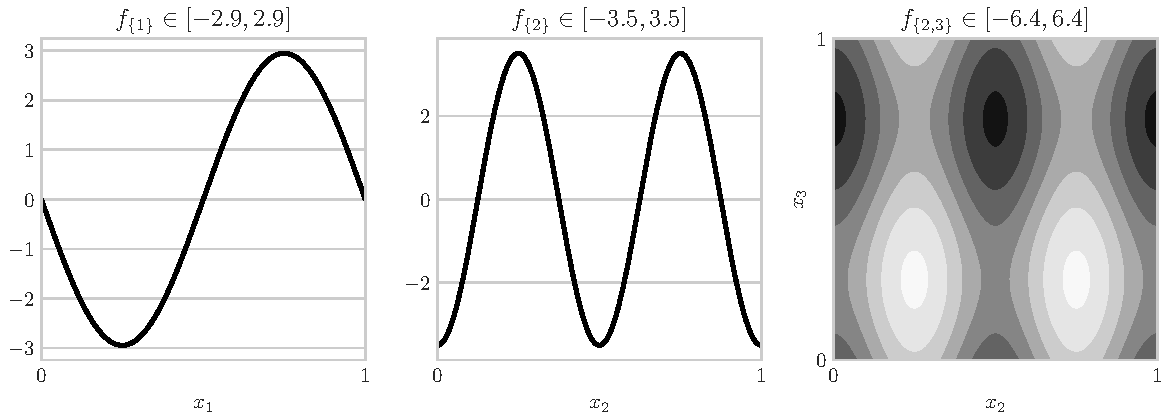
\includegraphics[width=.8\textwidth]{figs/ishigami_fu.pdf}
    \caption{Select analytic Ishigami sub-functions $f_u$ for some $u \subseteq 1:d$ from \eqref{eq:fanova}.}
    \label{fig:ishigami_fu}
\end{figure}

\begin{figure}[t]
    \centering
    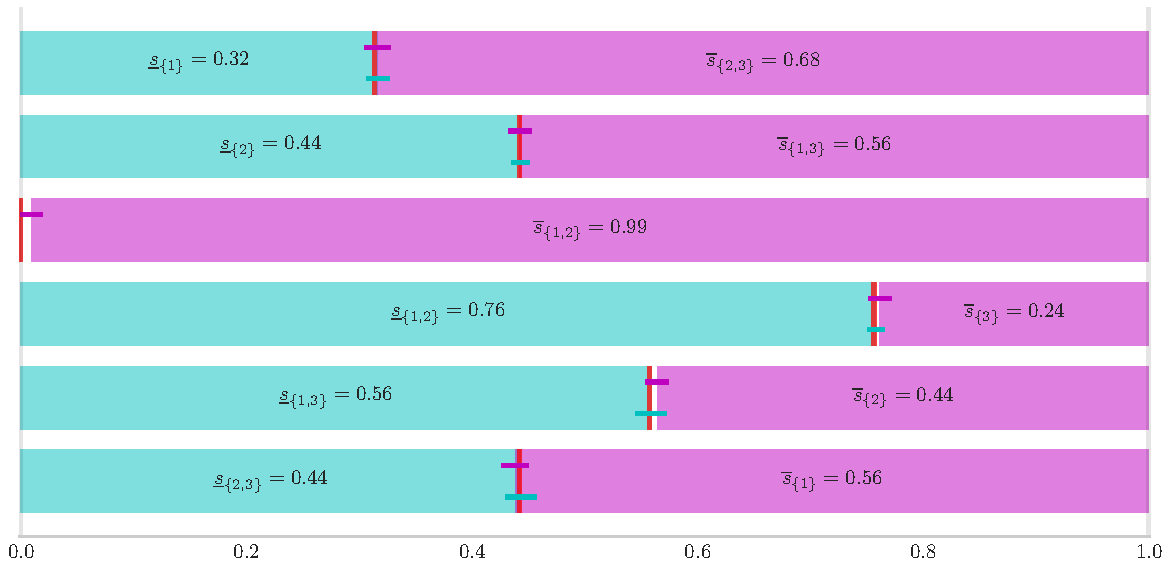
\includegraphics[width=.8\textwidth]{figs/ishigami.pdf}
    \caption{Approximate closed and total sensitivity indices for the Ishigami function illustrating the relationship $\underline{s}_u + \overline{s}_{u^c} = 1$ all $u \subseteq 1:d$. In each row the closed sensitivity index bar is  extended to the right from $0$ while the total sensitivity index bar is extended to the left from $1$. The bars should meet at the dark vertical line for the  analytic solution $\underline{s}_u=1-\overline{s}_{u^c}$. The darker,lighter horizontal lines within each row depict the error bounds for the closed, total sensitivity indices respectively. The vertical line crossing both horizontal lines in each row indicates the true solution is indeed captured in the error bounds as desired.}
    \label{fig:ishigami}
\end{figure}

\subsubsection{Neural Network Classifier of Iris Species}

In this example we compute sensitivity indices of a neural network classifier for the Iris dataset retrieved from the UCI Machine Learning Repository \cite{uci_ml_repo}. This example was inspired by a similar approximation in \cite{hoyt2021efficient}. The Iris dataset consists of input features
\begin{itemize}
    \item SL: sepal length (cm),
    \item SW: sepal width (cm),
    \item PL: petal length (cm),
    \item PW: petal width (cm)
\end{itemize}
from which an Iris is to be classified as either the \emph{setosa}, \emph{versicolor}, or \emph{virginica} species. We begin by fitting a neural network classifier \cite{he2015delving} which takes in input features and outputs a size $3$ vector of probabilities for each species summing to $1$. Taking the argument maximum among these three probabilities gives a species prediction. On a held out portion of the dataset the neural network attains 98\% classification accuracy and may therefore be deemed a high quality surrogate for the true relation between input features and species classification. 

Our problem is to quantify, for each species, the variability in the classification probability attributed to a set of inputs. In other words, we would like to compute the sensitivity indices for each species probability. In Listing \ref{py:nn} below we compute all sensitivity indices with the help of the scikit-learn package \cite{scikit-learn} for splitting off a holdout dataset and training the neural network classifier. Note that $\bd_{\bmu} = (2,3,14,3)$ and $\bd_{\bs} = (2,14,3)$ since we have $3$ classes, $14$ sensitivity indies of interest, and we are computing both the closed and total sensitivity indices. Figure \ref{fig:nn_si} visualizes closed sensitivity index approximations. 

\lstinputlisting[caption={Neural Network Sensitivity Indices},style=Python,label={py:nn}]{python/nn.txt}

\begin{figure}[t]
    \centering
    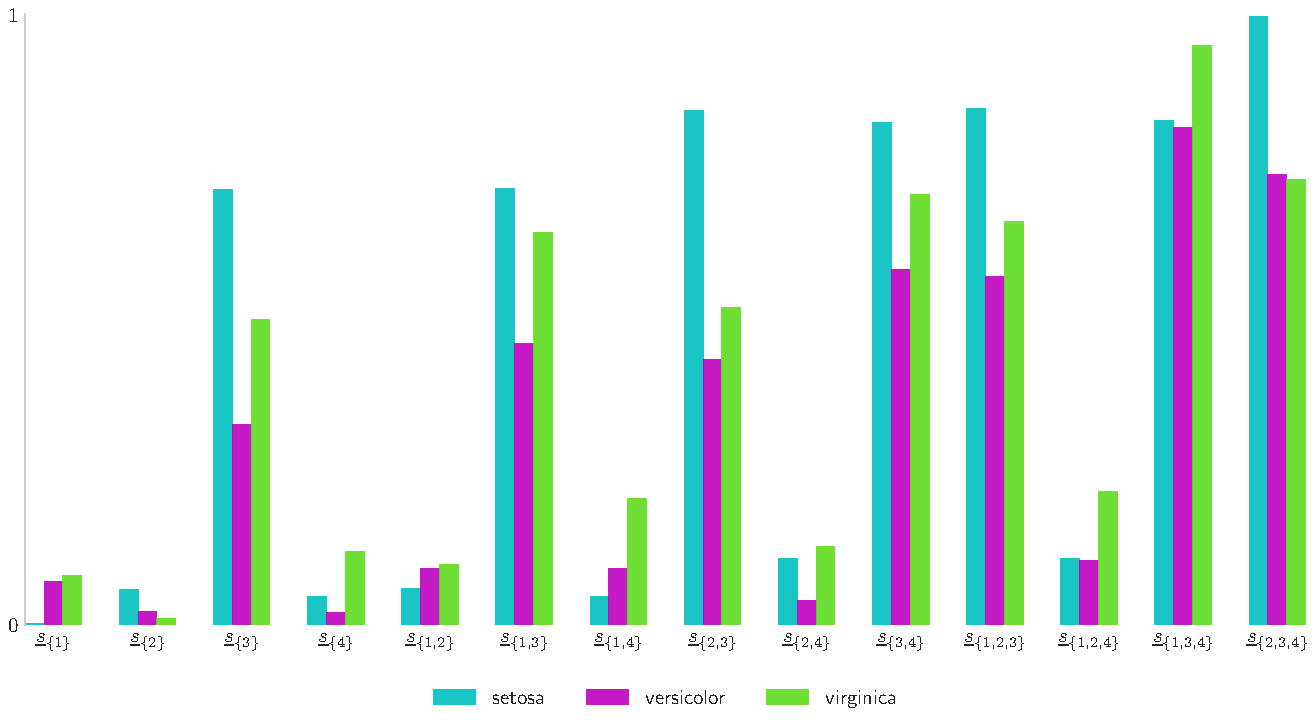
\includegraphics[width=.8\textwidth]{figs/nn_si.pdf}
    \caption{Closed sensitivity indices for neural network classification probability of each Iris species.}
    \label{fig:nn_si}
\end{figure}

\section{Conclusion} \label{sec:conclusions}

This article has extended adaptive MC and QMC stopping criteria to support multi-dimensional quantities of interest formulated as functions of multi-dimensional expectations. The resulting method is compatible with any algorithms providing error bounds holding with a desired uncertainty based on function evaluations at IID or LD sequences. Our work has been implemented into the open-source QMCPy package and exemplified on problems from machine learning. 

\printbibliography

\section*{TODO}

Create your own comment command with something like
\begin{verbatim}
    \texttt{\newcommand{\FJHComment}[1]{{\color{purple}#1}}}
\end{verbatim} 
Then when you add inline comments or comments below we know who made the suggestion. 

\subsection*{Article}

\begin{itemize}
    \item Remove "Listing ..." name for code we don't reference in the text 
\end{itemize}

\subsection*{Code}

\begin{itemize}
    \item \AGSNote{\texttt{CubBayes} algorithms allow ndarray of \texttt{abs\_tol} and \texttt{rel\_tol} and \texttt{error\_fun}}
    \item \AGSNote{New PyPI release}
    \item \AGSNote{update citation for demo reproducing figures in this article}
\end{itemize}

\end{document}
